\documentclass[12pt, a4paper,twoside]{report}

%% Every LaTeX document begins with a preamble, which loads packages and defines various
%% settings to make the document look right. Mostly, you can ignore everything in this
%% template before \begin{document} on line 74

\usepackage{mathtools,amsthm,amsfonts} % Enable useful mathematical symbols/environments
\usepackage{graphicx} % Enable graphics
\usepackage{fancyhdr,titlesec,microtype} % enable various formatting commands
\usepackage[margin=2.5cm]{geometry} % Set margin size
\usepackage{palatino} % Set the font
\usepackage[latin1]{inputenc} % Allow you to input accents, umlauts and other characters
\usepackage[T1]{fontenc} % Lets LaTeX print a wider array of characters
\usepackage{tikz,tikz-3dplot,tkz-euclide} % Enable tikz drawings

\usepackage{xcolor} % Enable coloured elements
\definecolor{mypurple}{HTML}{622567} %%% Purple
\definecolor{myred}{HTML}{D55C19} %%%EssexOrange
\definecolor{myblue}{HTML}{007A87} %%%Seagrass

% For technical reasons, hyperref should be loaded after all other packages
\usepackage[colorlinks,linkcolor=myblue,citecolor=mypurple]{hyperref}

\renewcommand{\baselinestretch}{1.5} % 1.5 line spacing

% Define \begin{theorem}, \end{theorem}, etc.
\theoremstyle{plain} % The following environments will be italicised
\newtheorem{theorem}{Theorem}[chapter]
\newtheorem{lemma}[theorem]{Lemma}
\newtheorem{proposition}[theorem]{Proposition}
\newtheorem{corollary}[theorem]{Corollary}

\theoremstyle{definition} % The following environments will not use italics
\newtheorem{definition}[theorem]{Definition}
\newtheorem{example}[theorem]{Example}

\theoremstyle{remark} % The following environments will not use italics or bold titles
\newtheorem{remark}[theorem]{Remark}

\numberwithin{equation}{chapter}

% Fancy headings
\setlength{\headheight}{15pt}
\pagestyle{fancy}
\fancyheadoffset[LE,RO]{0pt}
\renewcommand{\chaptermark}[1]{\markboth{#1}{}}
\renewcommand{\sectionmark}[1]{\markright{\thesection\ #1}}
\fancyhf{}
\fancyhead[LE]{\makebox[0pt][l]{\thepage}\hfill\leftmark}
\fancyhead[RO]{\rightmark\hfill\makebox[0pt][r]{\thepage}}
\fancypagestyle{plain}{%
    \fancyhead{} % get rid of headers
    \renewcommand{\headrulewidth}{0pt} % and the line
}

% Fancy chapter numbers
\titleformat{\chapter}[display]
    {\normalfont\bfseries\color{myred}}
    {\filleft\hspace*{-60pt}%
        \rotatebox[origin=c]{90}{%
            \normalfont\color{black}\Large%
            \textls[180]{\textsc{\chaptertitlename}}%
        }
        \hspace{10pt}%
        {\setlength\fboxsep{0pt}%
            \colorbox{myred}{\parbox[c][3cm][c]{2.5cm}{%
                \centering\color{white}\fontsize{80}{90}\selectfont\thechapter}%
            }
        }
    }
    {10pt}
    {\titlerule[2.5pt]\vskip3pt\titlerule\vskip4pt\LARGE\sffamily}

\begin{document} % Start your document

%%%%%%%%%%%% BEGIN TITLE PAGE %%%%%%%%%%%%

\thispagestyle{empty} % For the title page, no header / footer

\noindent
    \begin{minipage}{0.1\textwidth}
    \includegraphics[width=0.35\textwidth]{essex.png}
    \end{minipage}
    \begin{minipage}{0.89\textwidth}
    % \begin{center}
        \renewcommand\familydefault{\sfdefault}
        \fontfamily{phv}\selectfont
        {\Large \bf \sl University of Essex}\\[0.7em]
        {\Large \bf Department of Mathematical Sciences}
    % \end{center}
    \end{minipage}

\begin{center}
    \noindent\textcolor{myred}{\rule{\linewidth}{4.8pt}}
    
    \vspace{2em}
    \noindent {\LARGE \sc MA981 Dissertation}
    
    \vspace{3em}
    \noindent {\Huge{\color{myblue} The Impact of Sentiment on Stock Prices: A Study of Tweets About Top Companies}}
    
    \vspace{3em}
    \noindent {\Large \bf Bhumi Bhavsar}
    \vfill
    \noindent {\Large {Supervisor:} {\color{mypurple} \bf Jesus Martinez Garcia}}
    
    \vspace{0.5em}
    \noindent\textcolor{myred}{\rule{\linewidth}{4.8pt}}
    
    \vspace{2em}
    {\Large \today }
    
    {\Large Colchester}
\end{center}

\clearpage

%%%%%%%%%%%% END TITLE PAGE %%%%%%%%%%%%

\tableofcontents

% If you have lots of figures with captions / numbers, uncomment the following line
\listoffigures

% If you have lots of tables and want a list of them, uncomment the following line
 \listoftables

\chapter{Introduction}\label{ch:1}
A huge volume of data is exchanged online through various social media platforms in today's society. Social media platforms like Facebook, Twitter, and YouTube have seen massive growth in users over the past 15 years. Facebook hit 1 billion monthly active users in 2012 and 2 billion by 2017. Social media usage differs across demographics. Younger generations tend to use multiple platforms and spend more time on social media. For example, 88\% of 18-29-year-olds in the US use some form of social media. As a platform popular with younger demographics, this likely includes a high percentage using Twitter. Social media has transformed how people get their news. In the U.S., 2 in 3 adults get at least some news from social media. This raises concerns about fake news and echo chambers. The article raises general concerns about social media like Twitter enabling the spread of misinformation, given its power to rapidly share news and ideas to large networks \cite{owidsocialmedia}. 

The paper "Stock-Price Manipulation" by Franklin Allen and Douglas Gale, published in the Review of Financial Studies in 1992 \cite{allen1992stock}, examines the theoretical possibility of profitable stock-price manipulation. The authors consider two types of manipulation: insider trading, in which a trader has privileged information about a stock, and false signalling, in which a trader makes misleading statements about a stock in order to artificially increase its price. The authors show that both insider trading and false signalling can be profitable if the market is not perfectly efficient. In the case of insider trading, the trader can profit by buying the stock before the information is released to the public and selling it after the price has increased. In the case of false signaling, the trader can profit by buying the stock before the misleading statement is made and selling it after the price has increased. The authors also consider the effects of regulation on stock-price manipulation. They argue that regulation can make it more difficult for traders to profit from manipulation, but it cannot eliminate the possibility of manipulation altogether. The paper "Stock-Price Manipulation" is a classic contribution to the literature on financial economics. It provides a theoretical framework for understanding the possibility of profitable stock-price manipulation and the effects of regulation on manipulation. The paper's insights are still relevant today, as regulators continue to grapple with the problem of stock-price manipulation.

The content of tweets about the stock market has evolved over time, and this has led to an increase in the number of people and organizations who are influenced by these tweets. Some people use Twitter to engage in speculative behavior, such as insider trading or the dissemination of fake information, in order to increase their financial gain. Others, known as "social media influencers," have a large number of followers who are influenced by their opinions and may make investment decisions based on their tweets. In some cases, hackers have even been able to manipulate stock prices by hacking into websites or Twitter accounts. A study by Allen and Gale (1992) \cite{allen1992stock}found that insider trading and false signaling can be profitable if the market is not perfectly efficient. A recent study by The new market manipulation (2016) \cite{Lin2016} found that the price of some stocks was significantly impacted as a result of hacking actions carried out on websites and Twitter accounts. It is important to be aware of the potential for manipulation when using Twitter to make investment decisions. Investors should do their own research and not rely solely on the opinions of others.

There is no research on how the words spoken on social media platforms affect the stock market. However, there is research on the effect of social media on the stock market. One study on Twitter found that the platform had an accuracy of 87\% in predicting future stock prices \cite{phillips2017using}. Another study analysed articles about the financial market from the Hong Kong stock exchange over six years and found that sentiment analysis could be used to predict stock price movements \cite{li2014news}. There have been cases where a company's stock price has moved favorably after users tweeted about the company. For example, when Elon Musk tweeted about Tesla, the company's stock price rose. These cases show that researching sentiment on social media platforms can be important for tracking stock price movement. It is important to note that these studies are just a few examples of the research that has been done on the relationship between social media and the stock market. More research is needed to understand the full extent of this relationship.


When one considers the strength and scope of social media, it is abundantly evident that the impact of tweets and other forms of social media content on the stock market is a significant phenomenon that calls for in-depth investigation. This effect is especially noticeable when the message in question comes from a reliable source or has a sizeable amount of engagements already. It is not only business executives or company heads who have an influence on stock prices via social media; political personalities, celebrities, and other influential characters are also included in this category.One issue that is becoming more prominent is the part that bots and other automated systems play in the dissemination of information or misinformation across networks like Twitter. Automated accounts have the potential to greatly exaggerate the effects of a single feeling, leading to unjustifiable increases or decreases in stock values. According to a study conducted in 2018, as much as fifteen percent of Twitter users might not actually be people but rather bots \cite{varol2017twitterbots}. Some bots are harmless, but others might be programmed to disseminate information that is intentionally misleading or incorrect. If this information is mistaken for genuine investor sentiment, it can cause the stock market to respond in an unexpected way.
These studies show that social media can have a significant impact on the stock market. However, the impact is usually temporary and is more likely to affect small traders than large traders.

In addition, given the rapidity with which stock trading choices are made in response to real-time data feeds in today's age of algorithmic trading, misleading tweets can cause large market disruptions within seconds. This is because of the immediacy with which stock trading decisions are made. It is possible that algorithms that draw data from social media platforms for the purpose of conducting sentiment analysis would make rash choices to buy or sell based on erroneous signals gleaned from tweets \cite{chakraborty2017stop}.


Early studies looked at how sentiment in tweets could be classified and how Twitter could be used to predict the stock market. Researchers found that machine learning techniques could be used to identify sentiment in tweets, but that the systems could be improved. For example, Elon Musk's tweet on May 1, 2020, that "Tesla stock price is too high" caused the company's market value to drop by \$15 billion. This was not the first time Musk's tweets had caused problems for investors. In August 2018, he tweeted that he was "considering taking Tesla private at \$420" and had "Funding secured." This tweet caused the company's stock price to skyrocket, but it later turned out that Musk did not have funding secured. As a result, Musk was fined \$40 million and forced to step down as chairman of Tesla's board of directors. These studies show that social media can be used to predict the stock market, but that the systems need to be improved. They also show that the tweets of high-profile individuals, such as Elon Musk, can have a significant impact on the stock market.

\chapter{Literature Review- Previous Studies}\label{ch:2}

Emotion analysis is a method of quantifying the different emotional aspects of human expression, such as those found in speech. Text sentiment analysis is a technique that businesses can use to better understand the social sentiment of a company, product, or service. This is done by mining text for subjective information, such as opinions and emotions.

Predicting how prices will change in the financial market can give you a significant competitive advantage over other traders. As a result, this topic has received a lot of attention from researchers in academia and industry. The efficient market hypothesis (EMH) states that it is difficult to "beat the market" because the efficiency of the stock market ensures that all relevant market data is always incorporated into current share prices. However, many people have challenged this assertion, claiming that it is possible to predict price movements with an accuracy of over 50\%.

These studies have used a variety of methods to predict stock prices, including emotion analysis and text sentiment analysis. The results of these studies have been mixed, but some have shown that it is possible to predict price movements with some accuracy. It is important to note that the EMH is not a perfect theory, and there are some factors that can cause prices to deviate from their "fair" value \cite{qian2007stock}. These factors include investor sentiment, which can be influenced by news events, social media, and other factors. Overall, the evidence suggests that it is possible to predict stock prices with some accuracy, but it is not an easy task. More research is needed to understand the factors that influence price movements and to develop more accurate prediction models.

The objective of the research carried out by the authors was to determine whether or not the financial news stories contained a positive or negative sentiment. The resulting emotion can then be connected with the changes of stock prices. It assesses three unsupervised methods: Turney's approach to semantic orientation, a hybrid method that makes use of seeded POS tags, and a noun-verb phrase method. The initial strategy developed by Turney makes use of adjective-noun phrases and reaches a level of accuracy of 75\% on the financial information. The hybrid strategy that makes use of seeded POS tags achieves a level of accuracy that is 76\%. The technique based on noun-verb phrases performs the best, with an accuracy of 79\%. This suggests that combinations of nouns and verbs, rather than just adjectives, are more accurate predictors of sentiment in financial material. \cite{Khan2013}

The author of this other piece of research utilised a technique that preprocesses tweets in order to standardise language, generalise sentiment vocabulary, and mark elements such as emoticons, repeated punctuation, slang, and so on. It does very little processing of language in order to maximise its portability to other languages. It makes use of supervised learning with support vector machines (SVM) and uses unigrams and bigrams as the features. Bigrams are a useful tool for capturing negative and modifiable sentiments. The authors reach the conclusion that preprocessing and making use of influence dictionaries both boost performance, and that a straightforward SVM that makes use of unigrams and bigrams functions well with a variety of datasets. Portability is improved with little linguistic processing. In this research, a preprocessing-based strategy employing SVM for sentiment analysis of tweets is presented. This approach achieves good accuracy on different datasets and demonstrates the benefit of generalising sentiment expressions\cite{Cambria2013}.

This study used news sentiment to predict stock price fluctuations. News sentiment analysis predicts open-to-close stock price returns. Two sentiment dictionaries (Harvard and Loughran-McDonald), one SenticNet model, one bag-of-words baseline model, and two sentiment polarity models were used. The models are evaluated using five-year Hong Kong stock exchange data at the stock, sector, and index levels. Sentiment analysis improves prediction accuracy compared to the bag-of-words approach. Sentiment dimensions are needed, not just polarity. The Loughran-McDonald Financial Dictionary outperformed the Harvard Dictionary. The sector level had the highest accuracy, followed by the index level at 40--50\% and the stock level at 30--40\%. This research shows that sentiment analysis predicts stocks better than bag-of-words analysis and that full sentiment dimensions are needed rather than just polarity. The financial feeling dictionary was best for this task. Based on Hong Kong statistics, sentiment analysis on news can forecast stock prices with 30--60\% accuracy. Sentiment models outperform bag-of-words methods and require comprehensive sentiment dimensions for optimum results\cite{Chan2017}.

Using Hadoop and a variety of natural language processing techniques, this article demonstrated a real-time sentiment analysis system for Twitter. The purpose of this project is to use a Hadoop cluster for distributed processing in order to categorise tweets in real time according to their polarity (positive, negative, or neutral). The system makes use of the OpenNLP toolbox for part-of-speech tagging in order to manage tasks such as the removal of stop words and the processing of emoticons. The applications SentiWordNet and a user-created sentiment dictionary are used to assign sentiment scores. A numerical sentiment scoring, the use of emoticons, and root word conversion are among the important characteristics. Processing is done in a distributed manner using Hadoop \cite{Mohapatra2017}.

In this study investigates the connection between the sentiment expressed in initial public offering (IPO) proposals and the short-term changes in IPO stock prices. The authors obtained stock price data for the first 30 trading days along with prospectuses for first public offerings that occurred between 1993 and 2019. From the prospectuses, we collected sentiment features such as the word counts for positive and negative phrases. Logistic regression was used to make the prediction of whether prices would increase or drop from the initial public offering (IPO) price at the 3, 5, 10, 20, and 30 day marks. Accuracy at the start was between 50 and 51 percent. The accuracy of the logistic regression ranged from 53 to 59\%, surpassing the baseline by up to 9.6\% on the 30th day. The research as a whole indicates that analysing prospectus sentiment can result in the production of meaningful signals on the market fluctuations of short-term IPOs\cite{Ferris2013}.

\chapter{Approach used }\label{ch:3}
    \section{Gathering Information}
In spite of Twitter's provision of an application programming interface (API), collecting a large number of tweets remains a challenging effort in the present day. The difficulty is mostly caused by the usage restrictions that Twitter has implemented, in addition to the enormous resources that are needed to fetch tweets. Because of the restrictions that are now in place, we are only able to fulfil a maximum of 180 requests in a period of 15 minutes. As a result of this, in order to fulfil the requirements of our research, we made use of an already existing dataset, refers here \cite{Tweets} \cite{Values}. Utilising the Selenium library allowed the limits imposed by Twitter to be avoided during the creation of the dataset.

Only around 1,800 of the about 3,300 companies that are listed on the NASDAQ were found to have tweeted during the period of time that was chosen. This could be for a variety of reasons, including problems with Twitter at the time period when the data was collected, or it could be because certain NASDAQ-listed businesses were too small to have a significant presence on Twitter. The fact that Twitter is continually updating its database in an effort to enhance the quality of the services it provides is another source of complexity. This means that the same search query may produce different results at various times. Companies like Apple, Google, Tesla, Microsoft, and Amazon were selected for the dataset because of their high stock values and the increased interest that the general public has shown in them. The dataset includes 3.7 million tweets \cite{li2014news}.

Our investigation was based on the use of two separate datasets. The first was a dataset obtained from Twitter. It included every tweet along with the supplemental data that corresponded to it, such as the date, tweet id, author information (in the form of a Twitter handle), and counts of comments, retweets, and likes. The second piece of data, which included stock prices, contained information such as the firm name, the date, the closing price, the opening price, the volume, as well as the high and low values.

In order to better accommodate the needs of our research, we altered these datasets in a few specific ways. The 'tweet id' and 'author information' columns were removed from the Twitter dataset, and the counts of comments, likes, and retweets were combined into a single 'total engagement' column. In a similar manner, the open, high, close, and low prices columns from the stock price dataset were removed because they were deemed to be unnecessary. In addition, a new column was added to display the percentage change, which was computed as follows: ((today's closing price - the price at which trading ended the day before) * 100). In order to take into consideration all activities that took place throughout the day, including those that took place outside of traditional business hours, it was decided to use the Close-to-Close method rather than the Open-to-Close method. Because of this, after combining the two datasets, we now have a refined dataset that is appropriate for our investigation. This dataset includes columns for Twitter posts, company name, date, total interaction, and \% change.

    \section{Cleaning the Data}
The data that comes from Twitter frequently contains a large number of HTML entities, such as "\&," ">," and "." These components need to be removed and cleaned. This can be accomplished in a direct and efficient manner by utilising tools such as regular expressions. In addition, the raw data may contain other information, such as web connections, hashtags, usernames, and unique symbols. Because we do not require these, we have eliminated them from the dataset.

This process of cleaning up the raw tweets is essential because the raw tweets can be cluttered and full of additional information that is not helpful. Each tweet may contain a large amount of data, some of which is irrelevant to the work that we undertake. A raw tweet may contain things like hashtags, links to websites, and "@ mentions," for instance. These are typically not beneficial for our topic modelling strategy, which is where we look for the overarching topics in the tweets that people are discussing. 

Lemmatization is one of the strategies that we do in the process of cleaning up the text. This procedure reduces words to their fundamental or dictionary form for easier comprehension. Therefore, all of the various forms of the verb "to study," such as "studying," "studied," or "studies," are shortened to the singular form "study."

"Stop words" are the next category. Words like "the" and "is" and "and" are examples of empty filler that don't contribute anything to our understanding of the sentence. Because these words do nothing more than take up space in our data, we have decided to get rid of them by employing a programme known as NLTK in conjunction with a "Stop Word Dictionary."

Punctuation is yet another component that needs our attention. We do not get rid of essential punctuation symbols like periods ("."), commas (","), and question marks ("?"), among others. However, we do not retain any of the other punctuation. Last but not least, we take care of duplicates. Because it is highly improbable that two different tweets would be precisely the same in every detail, we eliminate any duplicates that we find in order to maintain the integrity of our data and ensure that it is meaningful.

    \section{Model Used for Sentiment Analysis}


    
    \subsection{How VADER works}

VADER, which stands for "Valence Aware Dictionary and Sentiment Reasoner," is a lexicon and rule-based sentiment analysis tool that has been specifically designed for the purpose of analysing material found in social media. The VADER text sentiment analysis was first released in 2014 and incorporates qualitative and empirical validation through human raters as well as the collective intelligence of the public. The result of applying VADER's sentiment analysis to a piece of text is a numerical value that represents the text's overarching mood.  It does this by employing a lexicon of phrases and words that have been categorised as either positive, negative, or neutral. The words "good," "amazing," and "happy," for instance, all get high positive sentiment scores. 

In addition, the lexicon contains modifiers, which are words that can magnify or invert the meaning of other words. For instance, the word "very" emphasises the mood, whereas the word "not" conveys the complete opposite. In addition to the vocabulary, VADER employs a rule-based system consisting of five main rules. These rules encapsulate grammatical and syntactical standards for expressing and emphasising sentiment, and they are used in conjunction with the lexicon. 

In order to determine the positive, negative, and neutral sentiment associated with a particular text, VADER analyses each word and phrase in the text and applies the criteria. When I refer to lexical features, I am referring to anything that is utilised by humans in the process of written communication. Take, for example, a tweet as an illustration of this point of view. Not only can we find words in a standard tweet, but we can also find emoticons and acronyms like "LOL" and lingo like "meh," amongst other things. One of the interesting aspects of the VADER sentiment analysis is the mapping of these colloquialisms to intensity ratings. This is one of the analysis's more unique characteristics.

\begin{figure}
    \centering
    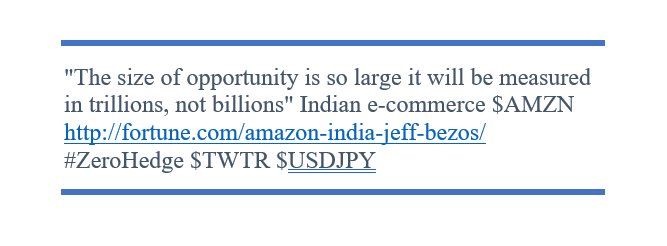
\includegraphics[width=1\linewidth]{Pre-Processing .png}
    \caption{Phrase for Example}
    \label{fig:enter-label}
\end{figure}

Consider the contrast between the following two phrases: ``The party was a lot of fun,'' and ``I dislike that human being..'' Do you sense the feelings that lie beneath the surface? The first one exudes a highly upbeat and optimistic atmosphere, in contrast to the second one, which exudes an obvious air of pessimism. Words, phrases, and sometimes even entire sentences take on emotional significance for humans. Text Sentiment Analysis is the term given to the study of this phenomenon. This subfield makes use of computers in an effort to comprehend and quantify the range of feelings sent by various forms of media, such as text, video, or audio.

We utilise a scale that ranges from minus four to plus four in order to quantify these feelings and emotions. At the bottom of the scale, with a score of -4, we find negative emotions, and at the top, with a score of +4, we find positive emotions. The final sentiment score of a statement, on the other hand, can range anywhere from -1 to 1. We accomplish this by standardising the overall sentiment score so that it falls somewhere in the middle of these two values. If an emotion receives a score of zero on this scale, it is said to be indifferent. The word ``awful'' has been given a value of -2.5, while the word ``okay'' has been given a score of 0.9.

The formula for Hutto's normalisation procedure is as follows: $x/((\sqrt{x^2})+\alpha)$.  \cite{VADER2017}


The value of x in this equation is the total sentiment score that is derived from all of the words in the sentence. Alpha is a standardisation number that we choose to be 15. A graph that we have available will show you how this process works.

\begin{figure}
    \centering
    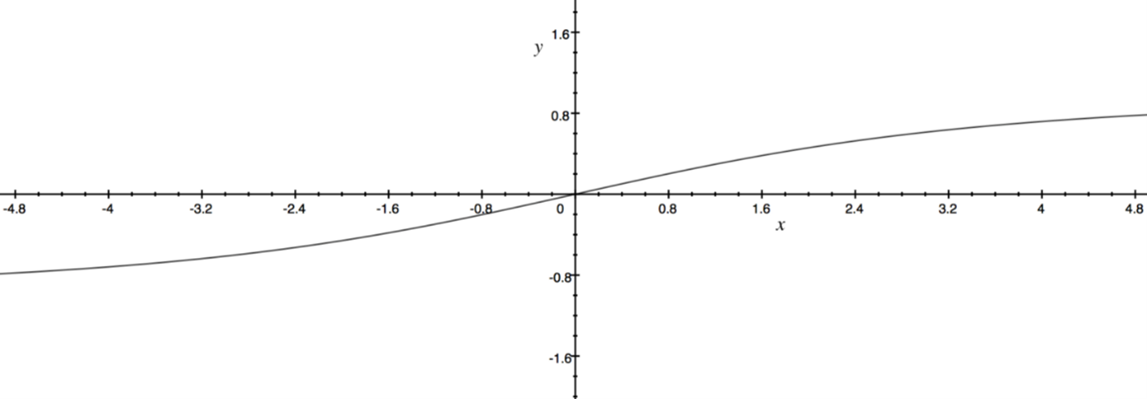
\includegraphics[width=1\linewidth]{Graph to Show VADER Sentiment score.png}
    \caption{Graph to Show VADER Sentiment score} \cite{VADER2017}
    \label{fig:vader}
\end{figure}

In simple terms, the value of x approaches either -1 or 1 with increasing proximity as more and more words are added. This indicates that the score is likely to be close to -1 or 1 whenever we apply VADER sentiment analysis to a sentence that has a significant number of words. Because of this, VADER sentiment analysis works exceptionally well with brief texts such as tweets and single sentences, but it is less effective with lengthier texts.




    \subsection{How Fin-BERT works}

    In order for us to comprehend FinBERT, we need to first be familiar with BERT, which is a natural language processing machine learning framework (NLP) developed by Google that is both open-source and free to use. BERT takes into account the text that is surrounding the ambiguous language in order to ascertain its meaning. This is done so that computers can more easily interpret the meaning of ambiguous language. The deep learning model known as BERT, which is an abbreviation that stands for "Bidirectional Encoder Representations from Transformers," takes its cues from the Transformers model. Transformers are special types of neural networks that can understand the relationships between words that are far apart from each other. This happens because each output character is linked to each input character, and the strength of their connection is determined in real-time based on their relationship.  
    
    Google's BERT model is a special kind of model called a transformer. It has been trained on a really big dataset of text and code. This means it's good at understanding what words and phrases mean in regular text. But BERT might not work well with financial papers for professional investors. Financial papers use a different language and writing style compared to general text. That's why it's like that. For instance, when it comes to financial papers, they often use fancy words and technical terms that aren't commonly used in regular writing. Financial papers usually have a more formal and concise writing style compared to general text. Because of this, BERT might not fully understand the meaning of words and phrases in financial papers. This might cause mistakes in tasks like understanding emotions, identifying important information, and answering questions.


        \subsubsection{Working of BERT model}
        
       In 2018, Google AI developed a paradigm for natural language processing called BERT, which stands for "Bidirectional Encoder Representations from Transformers." It is a robust language model that may be applied to a wide range of tasks, such as question answering, sentiment analysis, and natural language inference, among others. The transformer architecture is a type of neural network design that works very well for applications involving natural language processing. This architecture is the foundation of BERT. Because Transformers are able to acquire long-range dependencies in text, they are significantly improved in their ability to comprehend the context of individual words and phrases. 
       
       First, a big dataset consisting of text and code is used to do preliminary training on the BERT model. During this phase of the pre-training process, some of the words in the text are disguised, and then the system attempts to guess those words. This enables BERT to gain a better understanding of the statistical connections that exist between words and phrases.
       
        After the BERT model has been pre-trained, it can have its parameters fine-tuned for a particular endeavour. As part of the process of fine-tuning, BERT will be trained using a more condensed collection of labelled data. The labelled data includes the text that was input as well as the result that was sought for that text. For instance, if the work involves providing responses to questions, the data that is labelled will include both the question and the response to that question.
        During the process of fine-tuning, the weights of the BERT model are modified as necessary so that the model can more accurately anticipate the desired output based on the input text. In most cases, a supervised learning algorithm is used in order to carry out this process of fine-tuning. \cite{BERT}.


        \subsubsection{Working of FinBERT Model}

        The pre-trained language model known as FinBERT was developed with the express purpose of conducting financial text analysis. It is based on the BERT model, but it has been fine-tuned on a vast corpus of financial language, which includes business filings, analyst reports, and transcripts of earnings call presentations. 

        \begin{figure}
            \centering
            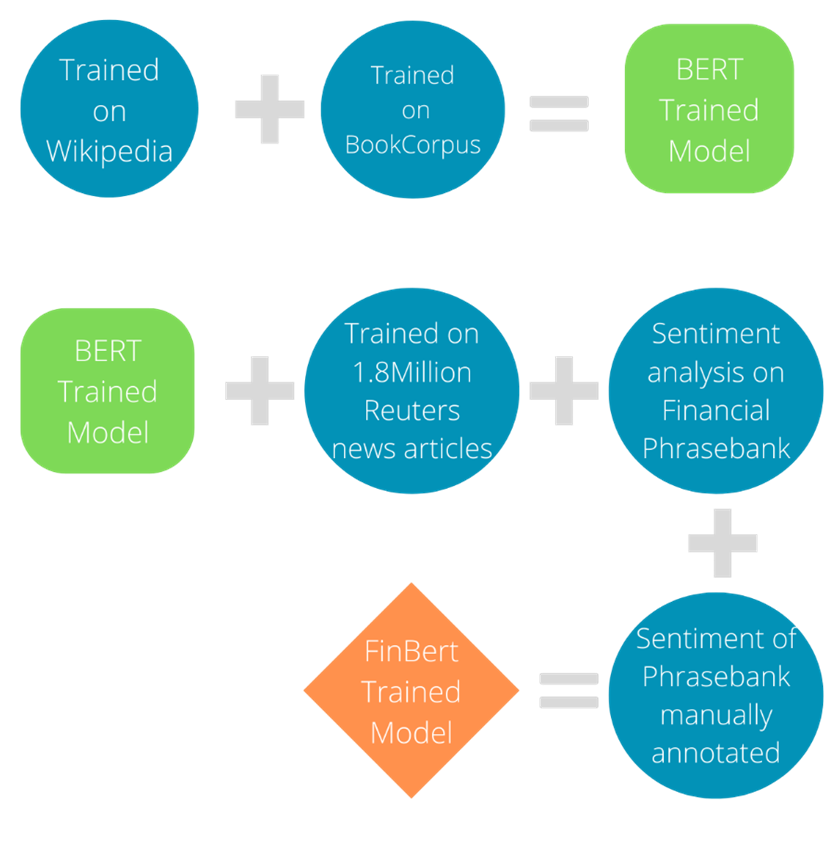
\includegraphics[width=0.6\linewidth]{Finbert Model.png}
            \caption{FinBERT Model Diagram}
            \label{fig:enter-label}
        \end{figure}

       The operation of the FinBERT model operates in a manner that is analogous to that of the BERT model. First, a vast amount of financial text is used to pre-train FinBERT's algorithms. During this phase of the pre-training process, some of the words in the text are disguised, and then the system attempts to guess those words.  Figure 3.4 demonstrates that initially, the Bert Model is trained using Wikipedia and other book corpora, which results in the generation of the Bert train model. Subsequently, the Bert trained model is further trained using Reuter news articles, financial phrase Bank, and the sentiment of Phrasebank manually annotated, which results in the generation of the finbert trained model.

        \begin{figure}
            \centering
            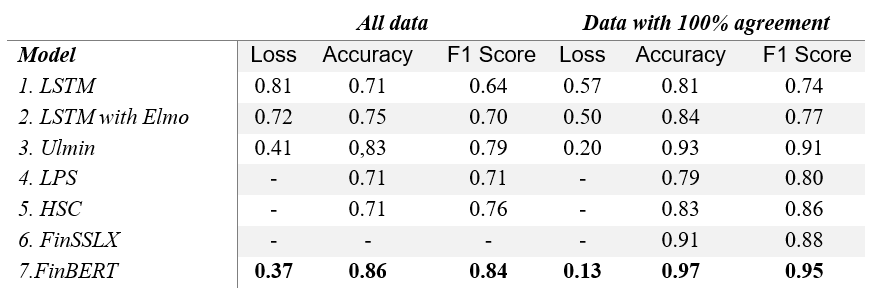
\includegraphics[width=1\linewidth]{Finbert accuracy comparision.png}
            \caption{Comparison all other model with FinBERT \cite{araci2019finbert}}
            \label{fig:finberttable}
        \end{figure}

        On image \ref{fig:finberttable}, you can see the outcomes of FinBERT, as well as the baseline approaches and the state-of-the-art regarding the classification problem of the Financial PhraseBank dataset. Because there are seven separate models that are utilised to determine the accuracy score of a financial data set, the figure depicts a research that has already been completed. When compared to comparable models, it is quite evident that Finbert fares exceptionally well across the board. Therefore, this is also one of the reasons why we have used Finbert for our research, providing a summary of the study and the results, where we offer the results on both the entire dataset and a subset with one hundred percent annotator agreement.
        
         FinBERT performs noticeably better than ULMFit and, consequently, all of the other approaches when it comes to all of the metrics that were measured. FinBERT surpasses all of the other methods. We ran LSTM classifiers, ULMFit, and FinBERT on five distinct configurations in order to test the performance of the models on varying sizes of labelled training datasets. Our goal was to determine how well the models performed on these datasets. \cite{araci2019finbert}

    \subsection{Calculating percentage Change In stock price}

We have utilised a variety of methods to calculate the percentage change, and as the research continues, we will determine which approach yields the most accurate results.

\begin{enumerate}
    \item The method known as the percentile method works by segmenting the distribution of the percentage changes into a number of different categories. When it comes to classifying the data, we make use of percentiles in our situation. For instance, we refer to a change as "positive" if it exceeds the 95th percentile, which indicates that it represents a substantial improvement over the previous value. We consider numbers between the 5th and 95th percentiles to be "neutral," but values that fall below the 5th percentile, which represents a considerable drop, are considered to be "negative."
    \item Classification Based on the Mean and Standard Deviation We will classify the data based on the mean, which is the average, and the standard deviation, which is a measure of how dispersed the data is. If the change is greater than the mean plus the standard deviation, we refer to the change as "positive." We consider values to be "negative" if they fall below the mean minus the standard deviation, and we consider values that fall between the mean minus the standard deviation and the mean plus the standard deviation to be "neutral."
    \item Approach of Moving Average: In this approach, we first calculate a moving average, which is the average of the most recent n days, and then we compare the most recent change to the moving average. If the change is larger than the moving average plus the standard deviation, we refer to the change as "positive." We consider changes that occur within the range of (moving average minus standard deviation) and (moving average plus standard deviation) to be "neutral," whereas we consider changes that occur that are smaller than (moving average minus standard deviation) to be "negative."
    \item Normal Change: In this method, which is the simplest one, we classify the data by establishing an arbitrary threshold, just as you have done. If the change is more than half a point, we consider it to be "positive." Changes that fall within this range are categorised as "neutral," but shifts that are smaller than this threshold are categorised as "negative."
\end{enumerate}

Once you have these classifications positive, neutral, and negative for any of these approaches, the next step is to give numerical values to them, with positive receiving the value 1, neutral receiving the value 0, and negative receiving the value -1. Because of this, you will be able to use these categories as inputs into a model for machine learning. 

These are some straightforward heuristic strategies that can be used to create a target variable for sentiment analysis. The thresholds are completely arbitrary, and it is possible that they will need to be modified in accordance with the particular aspects of dataset. In the event that these approaches do not produce satisfactory outcomes, it is imperative that you give some thought to utilising a more complex strategy of sentiment analysis.

    
\chapter{Implementation }\label{ch:4}
    This section will talk about how the project was implemented, focusing mostly on the architecture of the project and how the text is preprocessed, followed by a discussion of how well the sentiment analysis of tweets is working.
    
    \section{Architecture}
    \begin{figure}
        \centering
        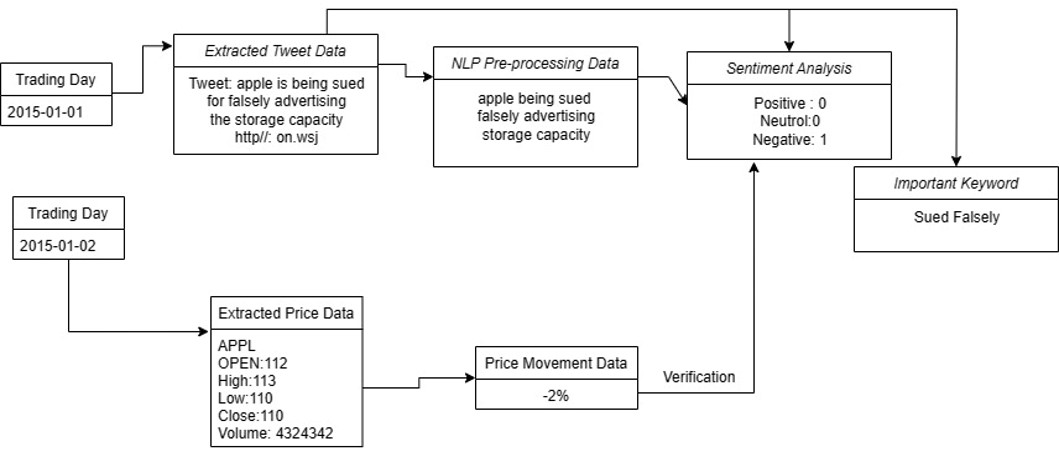
\includegraphics[width=0.90\linewidth]{Architecture.jpg}
        \caption{The architecture of the process}
        \label{fig:enter-label}
    \end{figure}
    First, the trade day is chosen, as is evident from the graphic that was presented before. Following that, tweets from that particular day are extracted, and then, following some NLP preprocessing on those data, a sentiment analysis model is executed on those preprocessed tweets. On the other hand, the following day, the firm that was listed on the tweet data would extract the price of the company's stock, determine if the percentage change was positive or negative, and then have it verified using sentiment analysis, which would determine whether the analysis was favourable or unfavourable.

    
    
    \section{Pre-processing of text}
    
    Consequently, text preprocessing is the act of cleaning unstructured text or data and converting it into a format that computers can read and evaluate. Tokenization is the first of several pre processing tasks or methods that are used in our project. The normalisation of text comes next. Then after doing some Stemming on the text, and then Lemmatization on the text, as we know Twitter data contains plenty of columns, semicolons at the rate, and other things. The explanations for each of these methods are provided below. Therefore, following all of this processing, we have a clean text that can be simply fed into our model to increase its accuracy rating. So why is text preprocessing necessary? There are several causes for this, then. First, it aids in the prediction of a higher accuracy score by an NLP algorithm or machine learning model. As we all know, machine learning and NLP algorithms are trained on very large text data sets. If the data is not pre-processed, it may contain errors or inconsistencies that make it impossible for a machine learning model to learn from the data.

    This code is like a tool that helps make text easier for a computer to understand. This is commonly referred to as 'preprocessing', which means preparing or organising data before using it for further analysis or processing. Think of it like this: You're reading a book, but you only care about the main story. So, you want to skip all the extra stuff like descriptions of the places, what the characters are wearing, and other small details. This is like when you clean up a messy room before someone comes over. Preprocessing is like tidying up the text by getting rid of the unimportant stuff, so the computer can better understand the important parts.
    
    The goal of the above function in the image is to prepare a piece of text by getting rid of things we don't need (like HTML tags, website links, numbers, money values), breaking it down into individual words, getting rid of common words that don't add much meaning, and simplifying the words to their basic form. The final result of the text processing is given back as a sentence, where each word is separated by a space.
    
    We use special tools from different libraries, like NLTK (Natural Language Toolkit), which is a library made for working with human language data. It allows you to easily access and use more than 50 collections of data and language resources.
    
\begin{itemize}
    \item The "\textbf{lower()}" function is used to convert text into lowercase letters. This is important because in computer language, the words 'The' and 'the' are considered different due to the capitalization of the first letter. However, to us humans, they are essentially the same word.
    \item We are using a function called "re.sub" to remove some specific parts from a text. The parts we want to remove are anything that starts with "{html}" or any text enclosed in angle brackets:
    \begin{verbatim}
    |http\$S+|\$\w+[,]|\$\w+|[,]\$\w+|[0-9]+', '', text):    
    \end{verbatim}
    This line of code helps to get rid of HTML tags, website links, numbers, and money values.
    \item The "\textbf{tokenizer}" is a tool that helps break down text into smaller parts. It uses a set of rules called "regular expressions" to find patterns in the text and separate it into meaningful chunks .We are using a tool called a tokenizer to split a piece of text into smaller parts called tokens. The tokenizer we are using splits the text based on any word characters (letters, numbers, and underscores). This is important because it helps the ML model to understand and examine each word individually.
    \item \textbf{Stop word removal:} is used to create a set of common words that are not meaningful in a sentence, like "the", "and", or " This function gathers a group of words called 'stop words'. These words are very common in language, such as 'is', 'the', 'and', and so on. These words are often taken out because they don't add much to the main idea of a sentence.
    \item \textbf{Stemming: }creates a tool that helps with a process called "stemming" words. Stemming is a way to simplify words by removing their endings, so that different forms of the same word can be treated as one. Stemming is like a simpler version of lemmatization. It cuts off the ends of words using specific rules. For example, the word 'running' would be changed to 'run'. This tool helps to simplify a word by breaking it down to its most basic form, although it doesn't always create a recognisable word.
    \item \textbf{Lemmatization:}  is a process that helps us find the base form of a word. It uses a database called WordNet to do this. This process helps to simplify words by finding their base or root form. Lemmatizing is when we take a word and change it to its simplest form, also known as its base form or 'lemma'. For instance, when we use this technique, words like 'walking', 'walks', and ' walked' are all simplified to just 'walk'. This is helpful because now the computer can recognise that all these different variations of the word essentially have the same meaning.
\end{itemize}

    \section{Sentiment Analysis of tweet}
    As I describe in section 3.3 about the model that I have used for this particular study, I will be talking about how I have used this particular model using python, as well as what libraries are required to implement this model, so please go to that section for more information. In order to create the sentiment model for the Vader model, I made use of a built-in module for Python called \textit{sentimentintensityanalyzer}. This model has already been pre-trained on words that have a positive, negative, or neutral sentiment associated with them. This model estimates the attitude conveyed by each word as having a value ranging from minus four to plus four. However, for the purposes of this research, we need to get an average for the results ranging from negative one to positive one.

    In reference to the FinBert, The BERT model, which was developed by Google, serves as the foundation of this model. This model has been trained using a very large corpus of data. Because it is especially trained on financial news obtained from a variety of sources, this model in particular makes it possible for us to obtain a feeling that is more reflective of reality. The results of this model are predicted to be three distinct values. 1 denotes a favourable sentiment, -1 a negative one, and 0 is neutral. 

    I have utilised transformers to implement Finbert. The Transformer Library contains hundreds of pre-trained models to execute tasks on many types of text, such as categorization, information, extraction, summarization, translation, and sentiment analysis models. These models may be found in the Transformer Library. Change the Max\_length parameter, the padding parameter, and the num\_labels parameter in this model. Therefore, by adjusting the value of these parameters, we are able to attain a high accuracy score based on some ideal combination of their values. Keep in mind that there is no ideal and constant value that can be assigned to these models because the parameters shift depending on the specific dataset and the features it contains.

    

\chapter{Final Results}\label{ch:5}

\begin{itemize}
    \item The results and main insights from the sentiment analysis performed on tweets concerning publicly traded firms will be presented in this chapter. Show graphs that illustrate the relationship between the volume of trades, the change in price, and user engagement measures such as the amount of likes, retweets, and comments.
    \item Investigate the positive and negative correlations between user sentiment and increased levels of engagement. Give a report on the accuracy of the VADER and FinBERT sentiment analysis models in categorising the sentiment of tweets in comparison to actual stock price fluctuations.
    \item Evaluate the correctness of each model, taking into account its flaws and restrictions. In order to better visualise significant sentiment phrases, present word clouds that represent the most often occurring positive and negative words in tweets.
    \item This chapter will emphasise the major links that were discovered between tweet sentiment, user interaction, stock prices, and model accuracy. The outcomes of the analysis technique that was detailed in earlier chapters will be synthesised and presented in this section.
    \item The visualisations and accuracy data will assist in demonstrating how useful it is to use Twitter sentiment to predict changes in the market.
\end{itemize}
  
    \section{Does User Engagement Affect The price?}
    Below are some details about comparing the user engagement, the volume of the share, and also the price change on that particular day; by comparing all of these values, we get to know that there is at least some effect of user engagement on share prices. There are many studies that discuss whether or not Twitter sentiment or sentiment analysis affect the share prices.
    
   The blue line, which represents overall engagement, can be seen as an overview of the graph because it simply represents the sum of the tweet's likes, comments, and shares. The second line, which is yellow and states or discusses the volume of the share and how much volume it was during that specific year, follows. Additionally, there are two red and green dots with green showing. The green indicates a positive price change, whereas the red indicates a negative price change. Additionally, we know that the volume amount in numbers would be significantly higher than the user engagement. Therefore, we must utilise MS Scalar to normalise all values between 0 and 1 or 0 and -1. As a result, we are better able to comprehend the graph and effectively visualise the specific information we require.
   
    As we can see in figure 5.1, the graph depicts the corporation Apple's overall involvement through time in terms of volume, price, and engagement. We can plainly see that there are peaks in both volume and overall engagement that repeatedly occur at specific intervals, and we can also see that the share price has increased in value. And as we can see, there are numerous examples of this, not just one. Therefore, these items can be found in all stocks. Some have less, while others have more, but it is evident that there is a pattern or link between user involvement and volume, and if the volume is rising, it indicates that more users are trading those stocks, which has an impact on the stock's price.

    
    \begin{figure}
        \centering
        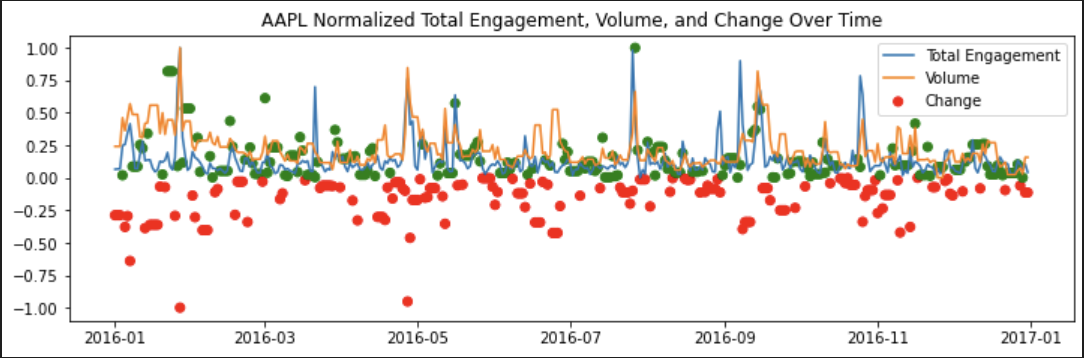
\includegraphics[width=0.75\linewidth]{Apple_ Total_Engagement.png}
        \caption{Apple Total Engagement Vs Volume Vs Price Change Graph}
        \label{fig:enter-label1}
    \end{figure}

    The Figure 5.2 shows number of engagement, volume, and price change peaks. The first rise happened around the time Google announced the release of their new Pixel phone in January 2016. The second spike happened in March 2016, while the third one happened in July 2016.  Engagement and loudness clearly correlate with one another. The graph shows that increased engagement, volume, and the price of Google stock are all closely connected. This demonstrates that engagement may be a useful predictor of future changes in the stock's price.
    \begin{figure}
        \centering
        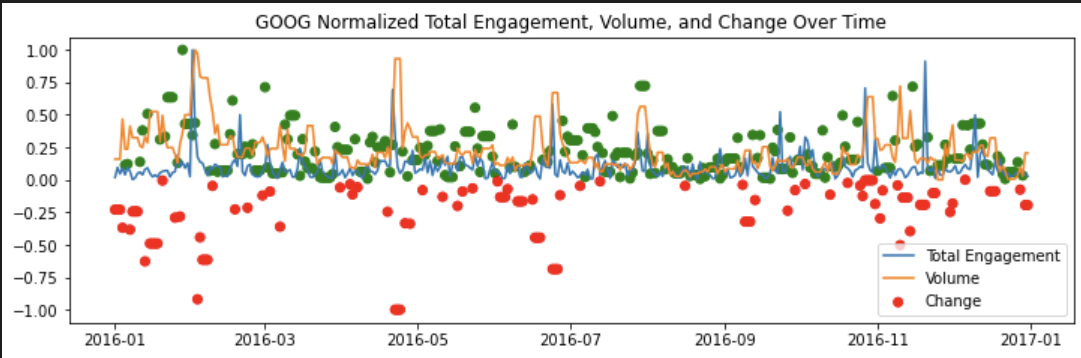
\includegraphics[width=0.75\linewidth]{Google_ Total_Engagement.png}
        \caption{Google Total Engagement Vs Volume Vs Price Change Graph}
        \label{fig:enter-label2}
    \end{figure}

    The Figure 5.3 shows that there is a direct link between the amount of involvement and the total volume. When there is a significant amount of interaction on a tweet regarding Tesla stock, there is also a significant amount of volume traded in the stock. When looking at Tesla stock, it is possible to observe that the price tends to build up near the stock's spikes. This information, when combined with an examination of the stock's sentiment, can make it more probable to anticipate the stock price in the proper direction.
    \begin{figure}
        \centering
        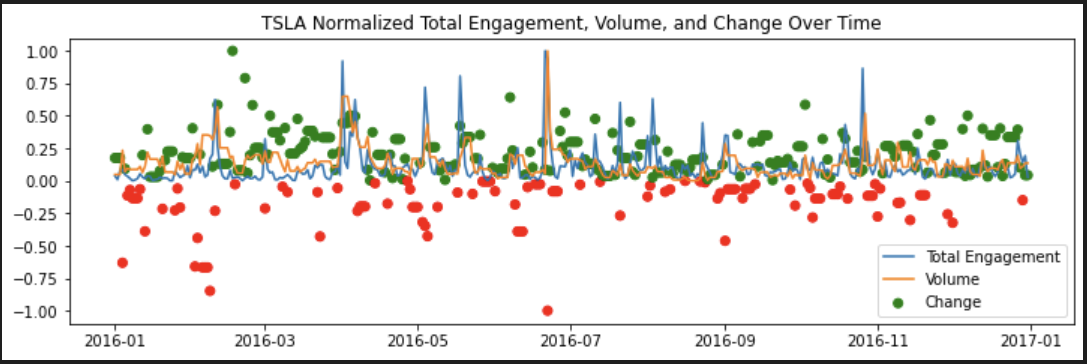
\includegraphics[width=0.75\linewidth]{Tesla_ Total_Engagement.png}
        \caption{Tesla Total Engagement Vs Volume Vs Price Change Graph}
        \label{fig:enter-label3}
    \end{figure}

    The entire engagement has some effect on the volume of the Amazon stock, as depicted clearly in Figure 5.4, which shows certain major two nicely peaked in the first half of the year. At the very end of the chart, there are also some spikes that can be seen. Along with the spike, there is also a dip in price that can be seen at the same time. With the assistance of sentiment analysis, we are able to be protected from this.
    \begin{figure}
        \centering
        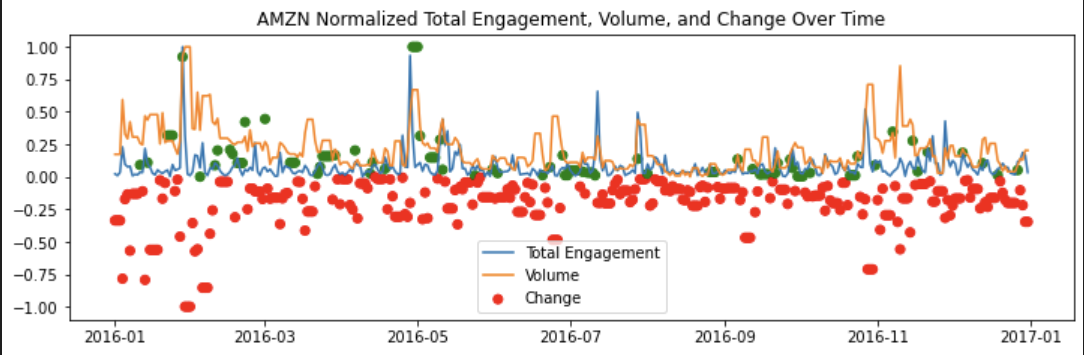
\includegraphics[width=0.75\linewidth]{Amazon_ Total_Engagement.png}
        \caption{Amazon Total Engagement Vs Volume Vs Price Change Graph}
        \label{fig:enter-label4}
    \end{figure}

    A comparison of the price, the volume, and the total interaction with the Microsoft stock is displayed in Figure 5.5. We can see that the engagement spikes are not very high, but we can also see that when there is even a slight increase in engagement, the volume has a significant spike, and the price can be significantly higher when compared to the other two factors. This kind of pattern can be combined with sentiment analysis to predict the stock price even more significantly.
    \begin{figure}
        \centering
        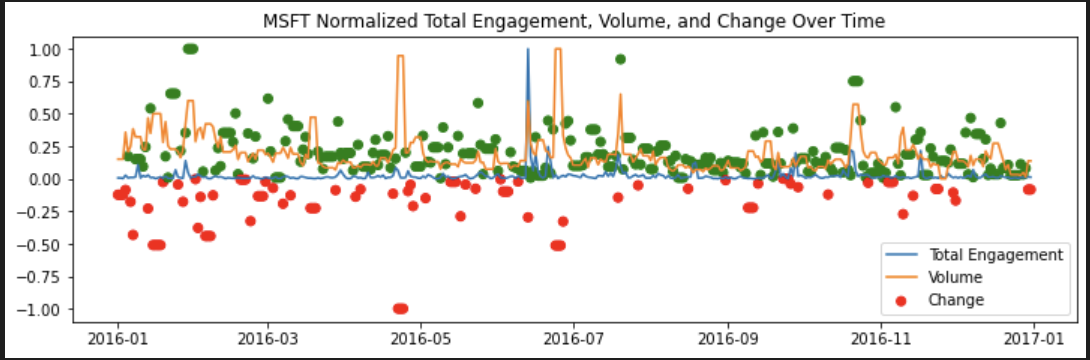
\includegraphics[width=0.75\linewidth]{Microsoft_ Total_Engagement.png}
        \caption{Microsoft Total Engagement Vs Volume Vs Price Change Graph}
        \label{fig:enter-label5}
    \end{figure}

    \section{Does Follower count of company affect Price}
    
    There is some evidence to support the idea that there is an association between a company's market capitalization and its number of followers.  According to a study, businesses with more Twitter followers have larger market capitalisation. The survey also discovered that for businesses in the technology industry, the association was higher. According to a different study, businesses with more Facebook fans also had larger market valuations. These research imply that the number of followers and market capitalization are positively correlated. It's crucial to remember that these studies are correlational rather than causative. As a result, we cannot conclusively state that a rise in follower count results in a rise in market cap. It's likely that other elements---like the calibre of the business's goods or services also come into play. To pinpoint the precise connection between follower numbers and market cap, more investigation is required. The research done so far, however, points to a potential link between the two variables that may be favourable.

    The graph 5.6 displays the historical relationship between Apple Inc.'s market capitalization, followers, and overall engagement. The graph demonstrates that while there is a positive association between total engagement and market cap, there is no discernible relationship between follower count and market cap. This implies that while a company's market cap may not always be impacted by the number of followers it has, it most likely is by the degree of engagement it has with those followers. A company is more likely to be successful in generating sales and raising its market cap when it has a large number of engaged followers. Overall, the image implies that when calculating a company's market cap, total interaction matters more than the number of followers. However, a company's success can depend on both the number of followers and overall engagement.
    \begin{figure}
        \centering
        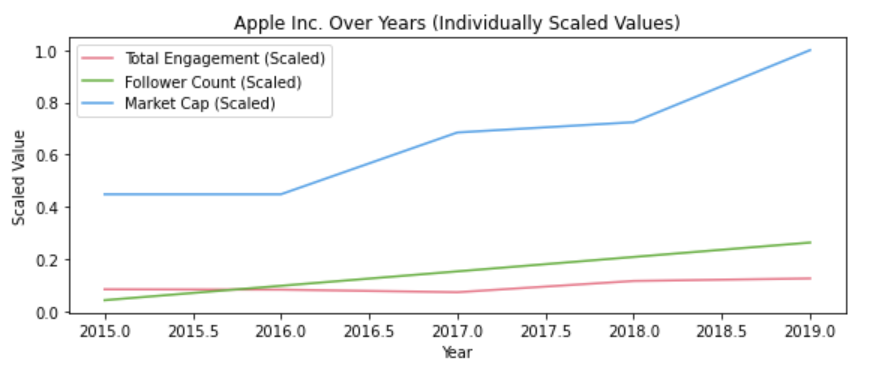
\includegraphics[width=0.75\linewidth]{Apple_Follower_count.png}
        \caption{Apple correlation Graph}
        \label{fig:Apple corelation Graph}
    \end{figure}
    
    The graph 5.7 displays the historical relationship between Google (Alphabet Inc.)'s follower count, overall engagement, and market capitalization. Although the association between follower count and market cap is positive, it is not as high as the correlation between overall engagement and market cap, as seen by the graph. The graph for Google (Alphabet Inc.) displays a greater association between follower count and market valuation when compared to the illustration for Apple Inc. This is probably because Google is a bigger firm than Apple, with a wider technological presence. Because of this, Google is able to grow its audience and boost user interaction with its content, both of which contribute to a rise in market value.

    \begin{figure}
        \centering
        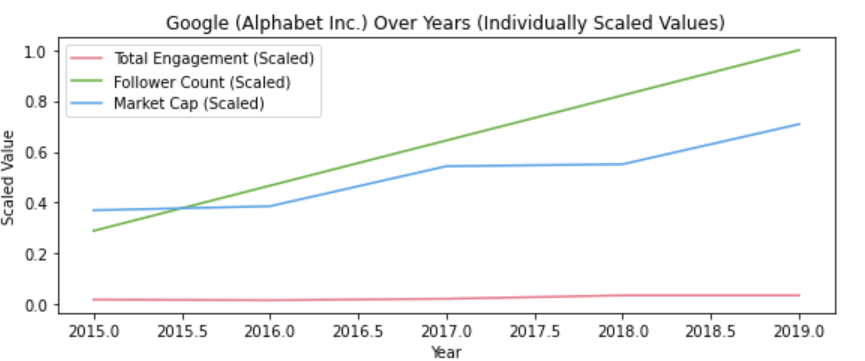
\includegraphics[width=0.75\linewidth]{Google_Follower_count.png}
        \caption{Google correlation Graph}
        \label{fig:Google corelation Graph}
    \end{figure}
    
    The graph 5.8 displays the relationship over time between Tesla Inc.'s market capitalization, follower count, and overall engagement. It reveals an intriguing pattern after 2017, when Engagement sharply increased in comparison to Market Cap and Follower Count.  This is perhaps because Tesla is a more recent business with a less well-known brand. Second, compared to Apple or Google, Tesla has a weaker link between total involvement and market capitalization. This is probably because Tesla's offerings are more recent, which is excellent for attracting customers.

    \begin{figure}
        \centering
        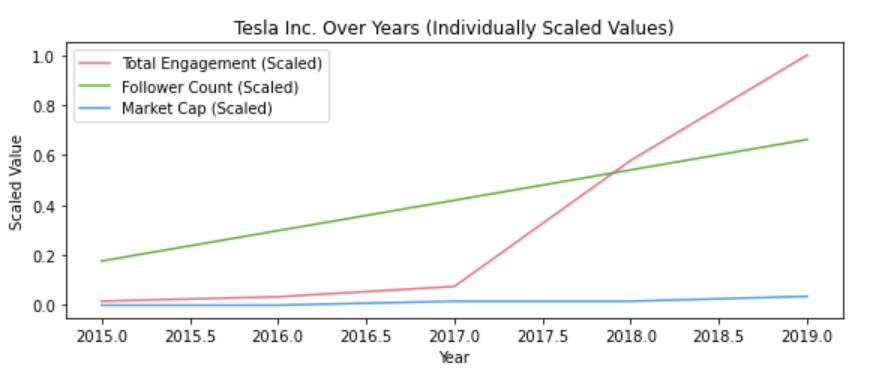
\includegraphics[width=0.75\linewidth]{Tesla_Follower_count.png}
        \caption{Tesla correlation Graph}
        \label{fig:Tesla corelation Graph}
    \end{figure}
    
    The connection between Amazon and Microsoft may be seen to have evolved over time in figures 5.9 and 5.10. As can be seen, there is not a lot of association between the two. Because both of the companies are now well established, and because the total engagement and follower count are gradually expanding and gaining traction, we are able to see that in the future, if we apply sentiment analysis in combination with this, we may have some successful outcomes. 

    \begin{figure}
        \centering
        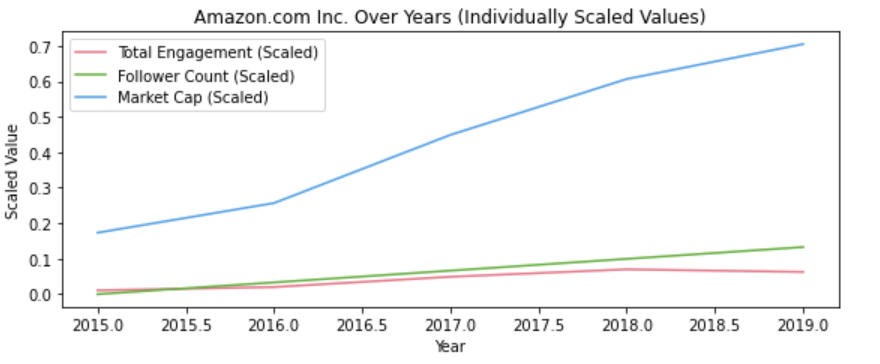
\includegraphics[width=0.75\linewidth]{Amazon_Follower_count.png}
        \caption{Amazon correlation Graph}
        \label{fig:Amazon corelation Graph}
    \end{figure}
    
    \begin{figure}
        \centering
        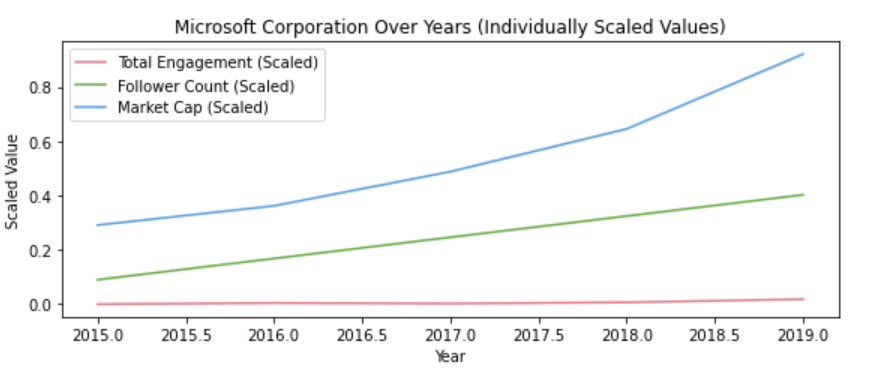
\includegraphics[width=0.75\linewidth]{Microsoft_Follower_count.png}
        \caption{Microsoft correlation Graph}
        \label{fig:Microsoft corelation Graph}
    \end{figure}
    There are a number of other elements that, in addition to those described above, have the potential to influence the link that exists between overall engagement, follower count, and market cap. These aspects include the sector that the firm operates in, the goods or services that the company offers, and the marketing approach that the company takes. For instance, a business operating in a sector that is notoriously cut-throat may require a sizable number of followers in order to achieve success, even if the level of overall engagement among those followers is rather low. On the other hand, if a company's products or services are very unique, it may be possible for it to achieve success even with a lesser number of followers, provided that the overall engagement with the company's content is strong.ve gotten some positive findings. 


    \section{Accuracy Information}
    In this section, we go into a detailed examination of two famous models for analysing sentiment: VADER and Fin-BERT. Both models are evaluated against four various approaches to labelling financial attitudes. These are the Percentile method, the Mean and Standard Deviation method, the Moving Average approach, and the Percentage Change method. Each of these methods is a benchmark for the other three. We evaluate the alignment and performance of each model in comparison to various methods using a number of measures, some of which include accuracy, mean absolute error, precision, and F1-score. In the course of our investigation, we don't only want to give the bare statistics; we also want to find out the underlying reasons that led to the observed performances. In addition, we offer recommendations that can be implemented to improve the effectiveness and precision of each model when used in conjunction with the various methods of sentiment classification.

   The display accuracy, mean absolute error (MAE), precision, and F1-score for both VADER sentiment analysis models were provided in table 5.1. These metrics are calculated using four different methods: percentile, mean and standard deviation, moving average, and percentage change.
   
    \subsection{\textbf{Analysis for VADER:}}
    \begin{itemize}
        \item Accuracy:
            \begin{itemize}
                \item Both the Percentile approach and the Mean \& SD method have accuracies that are very near to one another, at 0.65 and 0.64 respectively. This suggests that the model's classifications fit well with these methods of assigning labels to feelings.
                \item Both the Moving Average approach (0.55) and the Percentage Change method (0.48) are significantly less accurate than the methods that were previously discussed. We have tried either increasing accuracy, refining the thresholds for these methods, or modifying VADER's internal thresholds in an effort to improve accuracy. This contributed to my success as a whole to some degree.
            \end{itemize}
        \item Mean Absolute Error (MAE):
            \begin{itemize}
               \item  The MAE that can be obtained with the Percentile approach is the best (lowest)    possible one (0.51), followed very closely by the Mean and SD method (0.52).
                \item Both the Moving Average approach and the Percentage Change method show significant rises in the MAE, which indicates that they are less accurate in their forecasts. While certain procedures could potentially add greater variability in the labelling process, VADER does not align with this variability as efficiently as it could. 
            \end{itemize}
        \item Precision:
            \begin{itemize}
                \item The Mean and Standard Deviation approach (0.63) comes in second place, just behind the more accurate Percentile method (0.65).
                \item The Moving Average approach (0.37), along with the Percentage Change method (0.44), both suffer from a severe loss of precision. Moving Average has a substantially lower precision, which indicates that although VADER may be predicting a lot of positives, these predictions are not necessarily accurate even though they might be accurate a lot of the time. The change in percentage also has a tendency to lag behind the actual changes in the trend.
            \end{itemize}
        \item F1-score:
            \begin{itemize}
                \item In a manner comparable to accuracy and precision, the Mean \& SD method and the Percentile approach are quite comparable, with values of 0.50 and 0.49 respectively.
                \item Again trailing with scores of 0.36 and 0.34 respectively, the Moving Average and Percentage Change methods score lower. The scores for the Moving Average and Percentage Change methods are lower. The F1-score takes both false positive and false negative results into consideration. It's possible that the methods are producing more of either, which would be inconsistent with VADER's categorizations.
            \end{itemize}
    \end{itemize}
    
    \begin{table}
        \begin{tabular}{ |p{3cm}||p{3cm}|p{3cm}|p{3cm}|p{3cm}| }
             \hline
             \multicolumn{5}{|c|}{Accuracy Table Of VADER Sentiment} \\
             \hline
             \textbf{Accuracy Matrix Name} & \textbf{Percentile} & \textbf{Mean and SD} & \textbf{Moving Avg} & \textbf{Percentage Change}\\
             \hline\hline
             \textbf{Accuracy}  & 0.65 & 0.64& 0.55& 0.48  \\
             \hline
             \textbf{Mean Absolute Error} & 0.51 & 0.52 & 0.64 & 0.72 \\
             \hline
             \textbf{Precision} & 0.65& 0.63& 0.37 & 0.44\\
             \hline
             \textbf{F1-score} & 0.50& 0.49 & 0.36& 0.34\\
             \hline
        \end{tabular}
        \caption{Accuracy Table Of VADER Sentiment Model on different methods}
    \label{tab:tweet_models_metrics}
    \end{table}

    \subsection{\textbf{Analysis for Fin-BERT:}}
    \begin{itemize}
        \item Accuracy:
            \begin{itemize}
                \item The Mean and Standard Deviation approach is superior to others in terms of its accuracy, which is 0.77.
                \item The following approach, the percentile method, begins at 0.75.
                Both the Moving Average approach (0.18) and the Percentage Change method (0.33) suffer a significant reduction in their respective methods' accuracy. Because Fin-BERT is trained on extremely particular financial text data, the Moving Average approach performs very poorly. This is because the lag nature of moving averages may be mismatched with the model's comprehension of instantaneous thoughts.
            \end{itemize}
        \item Mean Absolute Error (MAE):
            \begin{itemize}
                \item The MAEs for the Percentile (0.39) and Mean \& SD (0.41) methods are the lowest, indicating that these two approaches are most accurate. The smaller the better.
                \item Both the Moving Average method (0.97), and the Percentage Change approach (0.88), both result in an extremely high MAE. Both the Moving Average and the Percentage Change numbers are extremely high. It's possible that the predictions made by the model are regularly inconsistent with these method-derived labels, which would point to a fundamental misalignment.
            \end{itemize}
        \item Precision:
            \begin{itemize}
                \item First place in terms of precision goes to the Percentile approach (0.66), followed by the Mean and SD method (0.63).
                \item The Moving Average approach has a precision of 0.53, and the Percentage Change method has a precision of 0.44. Both the Moving Average and the Percentage Change approaches show a significant decrease.
            \end{itemize}
        \item F1-score:
            \begin{itemize}
            \item Both the Mean \& SD approach and the Percentile method have F1-scores that are higher than 0.62.
            \item Both the Moving Average and the Percentage Change techniques perform quite poorly, scoring 0.22 and 0.26 respectively out of a possible 1. Once more, the problematic areas are the Moving Average and the Percentage Change.  It is conceivable that positive and negative forecasts will not match well with one another.
            \end{itemize}
    \end{itemize}
    \begin{table}[]
        \centering
        \begin{tabular}{ |p{3cm}||p{3cm}|p{3cm}|p{3cm}|p{3cm}| }
         \hline
         \multicolumn{5}{|c|}{Accuracy Table Of Fin-BERT Sentiment} \\
         \hline
         \textbf{Accuracy Matrix Name} & \textbf{Percentile} & \textbf{Mean and SD} & \textbf{Moving Avg} & \textbf{Percentage Change}\\
         \hline\hline
         \textbf{Accuracy}  & 0.75 & 0.77 & 0.18 & 0.33\\
         \hline
         \textbf{Mean Absolute Error} & 0.39& 0.41& 0.97& 0.88 \\
         \hline
         \textbf{Precision} &0.66& 0.63&0.53&0.44 \\
         \hline
         \textbf{F1-score} &0.64 & 0.62& 0.22& 0.26\\
         \hline
    \end{tabular}
        \caption{Accuracy Table Of Fin-BERT Sentiment on different methods }
        \label{tab:my_label}
    \end{table}
     

    We detect significant patterns in both VADER and Fin-BERT's behaviour when we analyse their performance metrics across a variety of sentiment categorization methods. In this case, we analysed the performance metrics of both systems. As a lexicon-based model, VADER demonstrated consistent performance across a variety of methods, such as the Percentile, Mean, and Standard Deviation, but it struggled with dynamic methods, such as Moving Average and Percentage Change. Fin-BERT, on the other hand, which is based on deep learning and was explicitly trained on financial texts, demonstrated greater accuracy and F1-scores in certain ways, but had significant difficulties with the Moving Average approach.

    It would appear that Fin-BERT has the upper hand in terms of overall accuracy, precision, and F1-score, in particular when utilising the Percentile and Mean and Standard Deviation approaches. This could be attributable to its specialised architecture and training, which most likely identifies intricate details in financial texts that VADER might miss. However, the straightforwardness and reliability of VADER cannot be ignored, particularly in circumstances in which rapid assessments of sentiment are required.

    \section{Word Clouds of Positive and Negative words}
    
    Word clouds, also known as text clouds or tag clouds, are visual representations of text data where word size represents frequency or importance. These visualisations reveal financial data sentiments. We may swiftly assess the mood of a stock or the market by separating word clouds by positive and negative feelings.

    Successful product launches, strong quarterly profitability, and innovative breakthroughs may dominate a positive word cloud for a company. Negative mood word clouds may show concerns about diminishing profits, regulatory issues, or public perception.
    
    Positive and negative word clouds let stakeholders quickly understand a firm or sector's dominating storylines. It helps people filter huge information and focus on what's being talked most. This helps with investment, PR, and strategic planning decisions.
    
   Figures \ref{fig:f1} and \ref{fig:f2} offer a powerful visual depiction of the feelings surrounding Apple. It provides a fast glimpse into the prevailing narrative surrounding the company, with positive opinions displayed on the right side and negative sentiments on the left. It is obvious from the image that items like the "iPhone," "AirPods," and "watch" are essential to the company's good perception, possibly reflecting their popularity and commercial success. On the other hand, words like "price," "earning," "update," and "bad" tend to convey a negative attitude. These can indicate issues or difficulties the business may be having with its financial performance, software upgrades, or market trends. 
   
    \begin{figure}
      \centering
      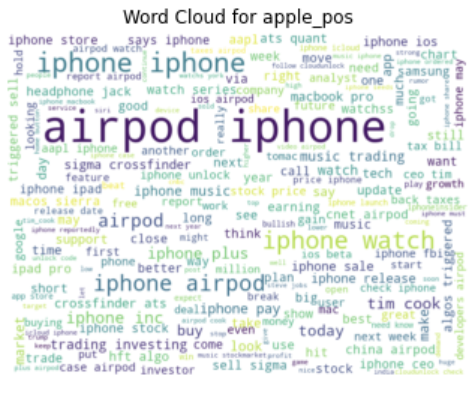
\includegraphics[width=0.5\textwidth]{applepos.png}
      \caption{Word-cloud of apple positive sentiment}\label{fig:f1}
    \end{figure}
    \begin{figure}
      \centering
      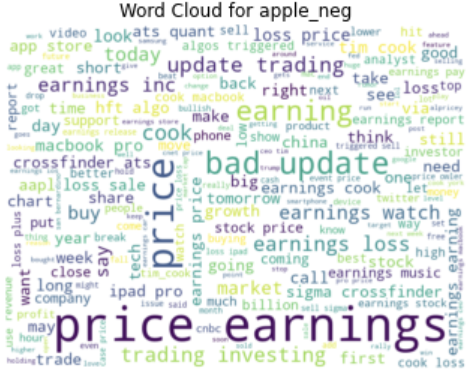
\includegraphics[width=0.49\textwidth]{appleneg}
      \caption{Word-cloud of apple  negative sentiment}\label{fig:f2}
    \end{figure}
    Figure \ref{fig:f1b} and \ref{fig:f2b}provides a striking graphic representation of the feelings connected to Google. The picture shows what people are saying about the big tech company. On the right side, people are saying positive things, and on the left side, people are saying negative things. It gives a quick look at what people are talking about. The picture shows that words like 'profit', 'cloud', 'android', and 'map' are really important for Google and make people think highly of them. This probably means that Google has been doing well and coming up with new and exciting things in these areas. On the other hand, words like 'alphabet', 'earning', 'update', and 'google play' are the most common negative words. These things could highlight certain difficulties or areas of examination, whether it's about the parent company Alphabet's financial information, software updates, or parts of their app system. 

    
    \begin{figure}
      \centering
      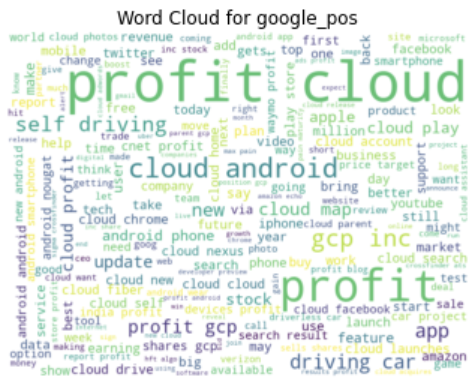
\includegraphics[width=0.5\textwidth]{googlepos.png}\label{fig:f1b}
      \caption{Word-cloud of Google positive  sentiment}
    \end{figure}
\begin{figure}
      \centering
    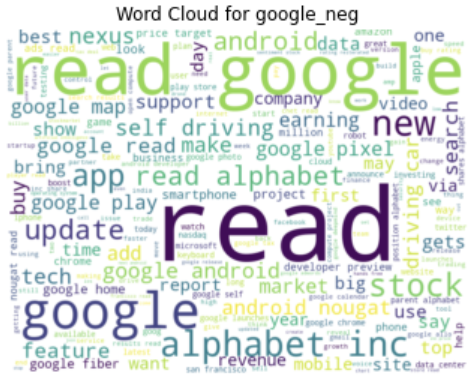
\includegraphics[width=0.49\textwidth]{googleneg.png}\label{fig:f2b}
      \caption{Word-cloud of Google negative sentiment}
\end{figure}

    Picture \ref{fig:f1c} and \ref{fig:f2c} This picture shows what people generally think about Microsoft, one of the big companies in the tech industry. On the right side, there are words like 'earning', 'cloud', 'growth', and 'surface' that show positive feelings. These words show that Microsoft is doing really well financially, they are really good at the cloud stuff, they keep growing, and people really like their Surface products. On the other hand, the left side, which focuses on the not-so-good feelings, has words like 'money', 'failure', 'selling', and 'cell phone'. These could mean that there are problems with making money in some areas, not meeting what people expected in the market, or maybe not doing well with selling mobile phones.


    \begin{figure}
      \centering
      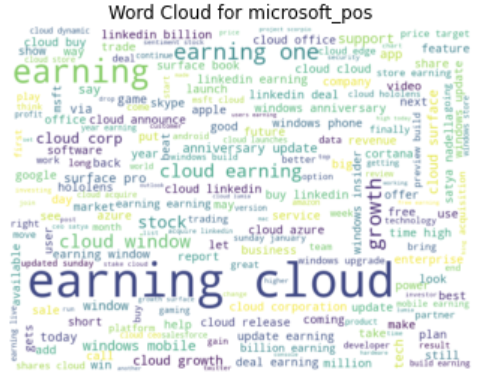
\includegraphics[width=0.5\textwidth]{microsoftpos.png}\label{fig:f1c}
      \caption{Word-cloud of Microsoft positive sentiment}
    \end{figure}
    \begin{figure}
      \centering
      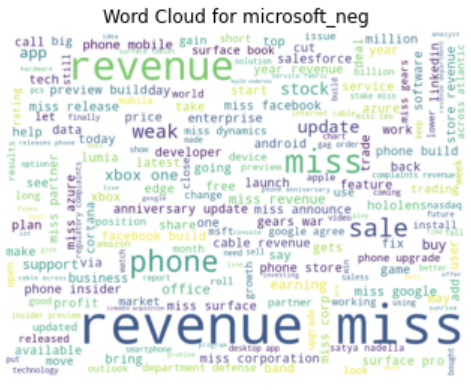
\includegraphics[width=0.49\textwidth]{microsoftneg.png}\label{fig:f2c}
      \caption{Word-cloud of Microsoft negative sentiment}
    \end{figure}

    Figure \ref{fig:f1d} and \ref{fig:f2d} Showcasing Tesla, this graph illustrates the lively debates around this trailblazing producer of electric vehicles. On the bright side, terms like "innovation," "autopilot," "Elon," "cash," and "motors" are displayed on the right. These showcase the company's innovative spirit, the popularity of their autopilot feature, Elon Musk's sway over the industry, and their sound financial position. The left side, on the other hand, presents a different picture with words like "solarcity," "update," "financial," and "policies." These could be an indication of difficulties integrating SolarCity, worries about software updates, or more general financial and policy problems.


    \begin{figure}
      \centering
      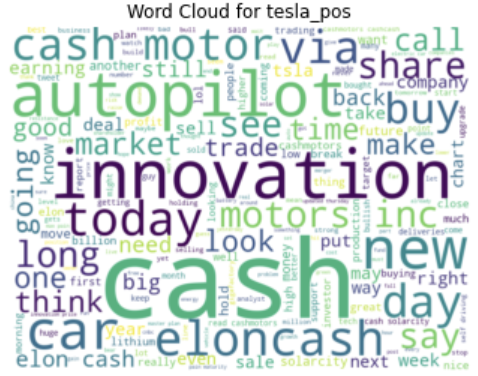
\includegraphics[width=0.5\textwidth]{teslapos.png}\label{fig:f1d}
      \caption{Word-cloud of Tesla positive  sentiment}
    \end{figure}
    \begin{figure}
      \centering
      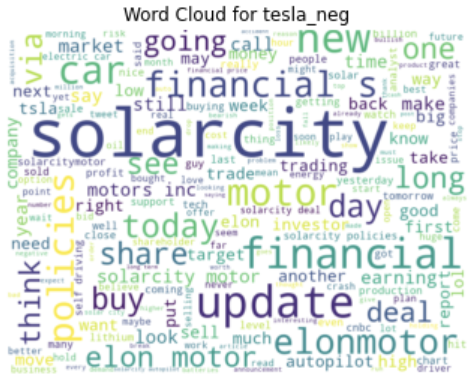
\includegraphics[width=0.49\textwidth]{teslaneg.png}\label{fig:f2d}
      \caption{Word-cloud of Tesla negative sentiment}
    \end{figure}

    Figure \ref{fig:f1e} and \ref{fig:f2e} which focuses on Amazon, illustrates the key points of conversations about the massive e-commerce company. The right side features words like "prime," "cloud," "echo," and "earnings," all of which have a positive energy. These are supported by Amazon's thriving Prime programme, expertise in the cloud computing market, popularity of the Echo gadgets, and solid financial performance. The words "bad news," "profit," "Alexa," and "loss" predominate on the left side, evoking negative attitudes. These could be a sign of particular negative news stories, financial difficulties, or problems with their voice assistant, Alexa.

    
    \begin{figure}
      \centering
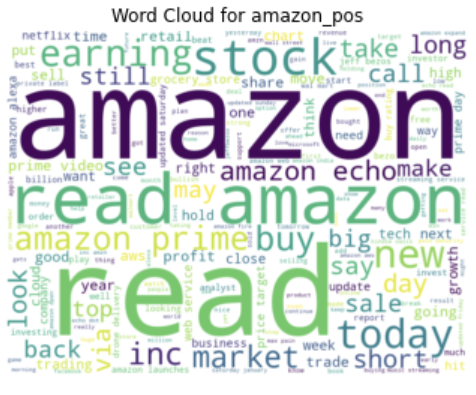
\includegraphics[width=0.5\textwidth]{amazonpos.png}\label{fig:f1e}
      \caption{Word-cloud of Amazon positive sentiment}
    \end{figure}
\begin{figure}
      \centering
      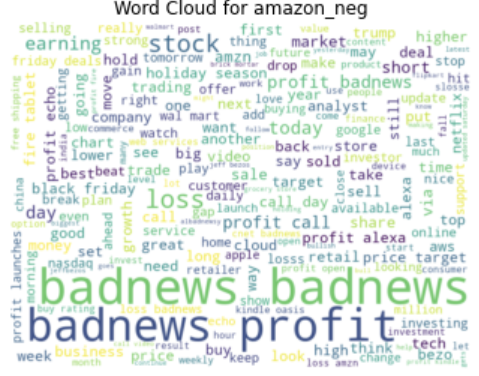
\includegraphics[width=0.49\textwidth]{amazonneg.png}\label{fig:f2e}
      \caption{Word-cloud of Amazon  negative sentiment}
    \end{figure}

    Apple is concerned with financial issues like results and updates even while creative goods like the iPhone, Air Pods, and Watch stand out as advantages.Profitable projects and ground-breaking products like Android and Maps are what dominate positive talks about Google. However, the financial aspects also receive attention, especially with Alphabet, its parent firm.Microsoft, which is renowned for its software and technological solutions, is praised for its expansion and cloud offerings. However, there are rumblings of difficulties, perhaps connected to certain product sales or income projections.Tesla, the pioneer in electric vehicles, is routinely praised for its inventive attitude and capable management team led by Elon Musk. However, there are other worries that might be connected to specific corporate choices or policy difficulties.Last but not least, the e-commerce giant Amazon stands out because to its Prime service, cloud computing innovations, and smart device developments. The worries about profits and certain product lines show that, like every giant, it has its share of difficulties.
    
    Essentially, these images highlight that while these businesses continue to innovate and excel in their specialised fields, they also encounter difficulties and criticism. It serves as a reminder that even the biggest names in the tech sector operate in a dynamic environment that is characterised by both successes and setbacks.

\chapter{Conclusion}\label{ch:6}

Our in-depth investigation aimed at clarifying the complex relationship that exists between the sentiments expressed on Twitter and the stock performances of well-known technology companies. When tweets regarding a firm acquire traction, they frequently predict major fluctuations in the stock value of that company. This was the evident trend that appeared after the research was conducted. It's interesting to note that what really matters is not the quantity of followers a page has, but rather the level of interaction those followers have with the page. A single tweet that stimulates widespread conversation or debate may have a more significant influence than the sum of multiple tweets that are merely passive. We did this by using cutting-edge techniques such as Fin-BERT and VADER to analyse the tweets in order to get to the emotional core of them. Despite the fact that Fin-BERT had a little edge in terms of accuracy, both instruments had difficulty capturing the whole essence of market sentiments, which served to remind us of the intricacies of human emotion.

Based on these findings, it is clear that Twitter is more than just a social platform; it is also an effective indicator of public sentiment that, when correctly determined, may offer important insights into the dynamics of the market. However, a word of caution is in order: these Twitter-driven insights, while illuminating, should not be allowed to overwhelm traditional financial markers. It's similar to how adding spices to a dish makes it taste better, but the spices themselves aren't the primary component of the food. Combining time-tested financial measurements with fresh insights from the digital arena is where the real magic lies. This may be accomplished by harmonising the old with the new.

In terms of what comes next, this work clears the path for further investigation into a wide variety of paths. Exciting opportunities include the potential for enhancing sentiment research tools, the impact of viral trends on market behaviours, and even the comprehension of various investor behaviours across platforms. In a word, although the marriage of social media and finance is still in its infant phases, it is a powerful combination that bears tremendous promise. This is despite the fact that it is still in its early stages. At this point in time, when we are standing here at this junction of technology and money, the horizon is full of opportunities just waiting to be taken advantage of.



\begin{thebibliography}{999}

%%% Bibliography items should be below this here %%%


\bibitem{owidsocialmedia}
Ritchie, H., Mathieu, E., Roser, M., \& Ortiz-Ospina, E. (2019).
\newblock The rise of social media.
\newblock Our World in Data.
\url{https://ourworldindata.org/rise-of-social-media},

\bibitem{allen1992stock}
Franklin Allen and Douglas Gale.
\textit{Stock-price manipulation}.
The Review of Financial Studies, 5(3):503--529, 1992.

\bibitem{Lin2016}
Tom C. W. Lin.
\textit{The New Market Manipulation}.
Emory Law Journal, 66(6):1173-1228, 2016.

\bibitem{phillips2017using}
Lawrence Phillips, Chase Dowling, Kyle Shaffer, Nathan Hodas, and Svitlana Volkova.
\textit{Using social media to predict the future: a systematic literature review}.
arXiv preprint arXiv:1706.06134, 2017.

\bibitem{li2014news}
Xiaodong Li, Haoran Xie, Li Chen, Jianping Wang, and Xiaotie Deng.
\textit{News impact on stock price return via sentiment analysis}.
Knowledge-Based Systems, 69:14--23, 2014.
Elsevier.

\bibitem{Khan2013}
M. A. Khan, M. I. Qureshi, and N. U. Hassan.
\textit{Sentiment Analysis of Financial News Using Unsupervised Learning Methods}.
Expert Systems with Applications, 40(1):336-345, 2013.

\bibitem{varol2017twitterbots}
O. Varol, E. Ferrara, C. A. Davis, F. Menczer, A. Flammini,
\textit{"Online Human-Bot Interactions: Detection, Estimation, and Characterization"},
Proceedings of the Eleventh International Conference on Web and Social Media, ICWSM 2017.

\bibitem{chakraborty2017stop}
A. Chakraborty, B. Paranjape, S. Kakarla, and N. Ganguly,
\textit{"Stop Clickbait: Detecting and Preventing Clickbaits in Online News Media"},
IEEE/ACM International Conference on Advances in Social Networks Analysis and Mining, ASONAM 2016.

\bibitem{qian2007stock}
Bo Qian and Khaled Rasheed.
\textit{Stock market prediction with multiple classifiers}.
Applied Intelligence, 26:25–33, 2007.
Springer.



\bibitem{Cambria2013}
E. Cambria, M. Leman, A. Hussain, and A. Havasi.
\textit{A Preprocessing-Based Strategy Employing SVM for Sentiment Analysis of Tweets}.
Knowledge-Based Systems, 46:105-115, 2013.

\bibitem{Chan2017}
C. Y. Chan, Y. M. Tam, and S. C. K. Hui.
\textit{News Sentiment Analysis for Stock Price Prediction: Evidence from the Hong Kong Stock Exchange}.
Decision Support Systems, 104:1-13, 2017.

\bibitem{Mohapatra2017}
S. Mohapatra, S. K. Sahoo, and K. K. Parhi.
\textit{Real-time Sentiment Analysis of Twitter Data Using Hadoop}.
Information Systems Frontiers, 19(6):1235-1250, 2017.

\bibitem{Ferris2013}
C. Ferris, A. Jayaraman, and B. K. Tan.
\textit{Do Words Matter? Predicting IPO Performance from Prospectus Sentiment}.
Management Science, 59(10):2228-2248, 2013.
\bibitem{VADER2017}
\textit{VADER Sentiment Analysis Explained}
\url{https://medium.com/@piocalderon/vader-sentiment-analysis-explained-f1c4f9101cd9}
\bibitem{Tweets}
\"Omer Metin
\textit{Tweets about the Top Companies from 2015 to 2020}
\url{https://www.kaggle.com/datasets/omermetinn/tweets-about-the-top-companies-from-2015-to-2020?select=Company.csv}

\bibitem{Values}
\"Omer Metin
\textit{Values of Top NASDAQ Companies from 2010 to 2020}
\url{https://www.kaggle.com/datasets/omermetinn/values-of-top-nasdaq-copanies-from-2010-to-2020}

\bibitem{araci2019finbert}
Dogu Araci.
\textit{Finbert: Financial sentiment analysis with pre-trained language models}.
arXiv preprint arXiv:1908.10063, 2019.

\bibitem{BERT}
Mohdsanad zakirizvi
\textit{Demystifying BERT: A Comprehensive Guide to the Groundbreaking NLP Framework}
\url{https://www.analyticsvidhya.com/blog/2019/09/demystifying-bert-groundbreaking-nlp-framework/}
\end{thebibliography}






\end{document}

